\documentclass[10pt]{beamer}

% handout
% \documentclass[handout, 10pt]{beamer}

\usepackage{clases}

\title{Investigacion Operativa}
\subtitle{Coloreo}
\date{}
\author{Facundo Gutiérrez - Nazareno Faillace}
\institute{Departamento de Matemática, FCEN, UBA}
% \titlegraphic{\hfill\includegraphics[height=1.5cm]{logo.pdf}}

\newcommand \anchoPagina{1.0} % El proyector no anda bien, hay que ajustar el ancho
\begin{document}

\maketitle

\begin{frame}{Coloreo - Definiciones}
	\begin{minipage}{\anchoPagina \textwidth}
	\textbf{$k$-coloreo} : un grafo admite un $k$-coloreo si existe una asignaci\'on de colores $\{1,\dots,k\}$ a los v\'ertices que cumple que todo par de v\'ertices vecinos tienen colores distintos.
	
	\vspace{1em}
	\pause
	\textbf{Número cromático ($\chi(G)$)} : es el menor $k$ para el cual $G$ admite un $k$-coloreo.

    \vspace{1em}
    \pause
    \textbf{clique} : es un subgrafo completo maximal.
    
    \vspace{1em}
    \pause
    $\omega(G)$ : tamaño de la clique más grande (clique máxima).
    
    \vspace{1em}
    \pause
    \textbf{Conjunto independiente} : es un subconjunto de v\'ertices para el cual no existe arista en el grafo original que conecte a ning\'un par de esos v\'ertices.
    
    \vspace{1em}
    \pause
    $\alpha(G)$ : tamaño del conjunto independiente máximo.

	\end{minipage}
\end{frame}

\begin{frame}{Coloreo - Propiedades Varias}
	\begin{minipage}{\anchoPagina \textwidth}
	    \footnotesize
	    \begin{tcolorbox}[title=Propiedades]
		\begin{enumerate}
			\item $\alpha(G) = \omega(\overline{G})$ 
			\item $\chi(G) \geq \omega(G)$
			\item $\chi(G) \leq \Delta(G) + 1$
			\item $\chi(G)\alpha(G) \geq |\mathbb{V}| $
			\item $\chi(G) + \alpha(G) \leq |\mathbb{V}|+1$ 
			\item $\chi(G) + \chi(\overline{G}) \leq |\mathbb{V}|+1$
		\end{enumerate}
		\end{tcolorbox}
		\vspace{0.4cm}
		\begin{tcolorbox}[title=Teorema de Brooks]
		Sea $G$ un grafo conexo. Entonces $G$ es $\Delta(G)$ coloreable, a no ser que ocurra alguna de las siguientes situaciones.
		\begin{itemize}
			\item $G$ es un grafo completo
			\item $G$ es un ciclo impar.
		\end{itemize}
		\end{tcolorbox}
	\end{minipage}
\end{frame}

\begin{frame}{Coloreo - Polinomio cromático}
        \small
		El \textit{polinomio crom\'atico} de un grafo $G$ es una funci\'on que se define por $P_{G}(k)$ como la cantidad de $k$-coloreos distintos que admite $G$
		
		Para ciertos grafos, calcular su polinomio cromático es bastante directo:
		\begin{itemize}
		    \item sea $\mathcal{N}_n$ el grafo nulo de $n$ vértices (i.e. $|\mathbb{V}|=n$, $|\mathbb{E}| = 0$), su polinomio cromático es: 
		    \visible<2>{\[ P_{\mathcal{N}_n}(k) = k^n\]}
		    \item sea $\mathcal{P}_n$ un camino simple de $n$ vértices, su polinomio cromático es:
		    \visible<2>{\[P_{\mathcal{P}_n}(k) = k(k-1)^{n-1}\]}
		    \item sea $\mathcal{K}_n$ el grafo completo de $n$ vértices, su polinomio cromático es:
		    \visible<2>{\[P_{\mathcal{K}_n}(k) = k(k-1)(k-2)(k-3)\dots(k-n+1)\]}
		\end{itemize}
		Sin embargo, no siempre es sencillo calcular el polinomio cromático de cualquier grafo a partir de sus propidades estructurales.
\end{frame}

\begin{frame}{Coloreo - Conexi\'on/Contracci\'on}
	\begin{minipage}{\anchoPagina \textwidth}
	    \footnotesize
		Dado un grafo $G$ y \textit{dos v\'ertices \underline{no adyacentes}}, digamos $u$ y $v$, definimos la \textit{conexi\'on} de $G$ por la arista $e = \
		\{u,v\}$ al grafo $G_1$ que resulta de agregar la arista $e$ a $G$. De manera similar, definimos la \textit{contracci\'on} de $G$ por $e = \{u,v\}$ al grafo $G_2$ que resulta de eliminar los v\'ertices $u$ y $v$ del grafo, y agregar un nuevo v\'ertice $uv$ que tiene como vecindario $\mathcal{N}(uv) = \mathcal{N}(u) \cup \mathcal{N}(v)$.
		
		\begin{figure}
		    \centering
		    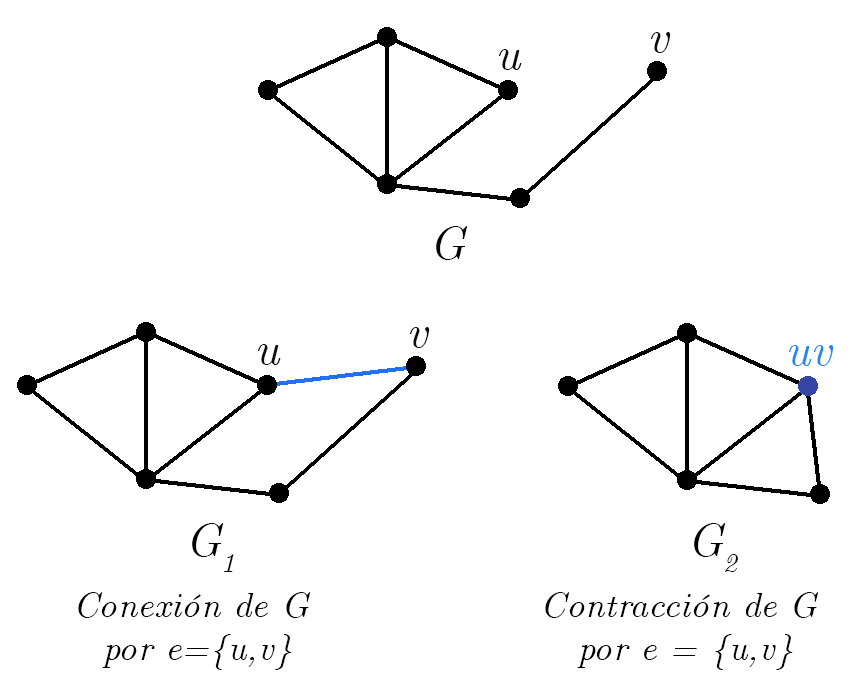
\includegraphics[scale=0.25]{imagenes/conexion-contraccion.jpg}
		\end{figure}

	\end{minipage}
\end{frame}

\begin{frame}{Coloreo - Conexi\'on/Contracci\'on}
	Teniendo esto en cuenta, se puede probar que valen las siguientes relaciones:
	\begin{enumerate}
		\item $\chi(G) = \min \{\chi(G_1),\chi(G_2)\}$
		\item $P_{G} = P_{G_1} + P_{G_2}$
	\end{enumerate}
	
	\pause
	Estos resultados dan las bases para el Algoritmo de conexi\'on contracci\'on tanto para coloreo como para hallar el polinomio crom\'atico.
\end{frame}


\begin{frame}{Coloreo - Conexi\'on/Contracci\'on}
	\begin{minipage}{\anchoPagina \textwidth}
	    \small
		La idea del Algoritmo de conexi\'on contracci\'on (también conocido como Algoritmo de Zykov) se basa en que sabemos resolver el problema para un grafo completo (los cuales ser\'an nuestros \textit{casos base}). Recordemos que en un grafo completo tenemos que:
		\pause
		\begin{itemize}
			\item $\chi(G) = |\mathbb{V}|$
			\item $P_{G}(k) = \prod\limits_{i = 0}^{|\mathbb{V}|-1} (k-i)$
		\end{itemize}
		Luego, como en cada conexi\'on se agrega una arista y en cada contracci\'on se elimina un v\'ertice, eventualmente llegamos a un caso base aplicando la recursi\'on dada por el resultado anterior.
		\pause
%
%		\textbf{Observaci\'on}:
%		\begin{itemize}
%% 			\item Podemos utilizar programaci\'on din\'amica para solo resolver una vez cada subproblema.
%			\item Podemos usar Branch \& Bound y utilizar el valor incumbente de la mejor soluci\'on obtenida hasta el momento para evitar ramificar.
%		\end{itemize}
	\end{minipage}
\end{frame}

\begin{frame}{Coloreo - Ejemplo de corrida del Algoritmo}
	\begin{minipage}{\anchoPagina \textwidth}
%		\begin{center}
%			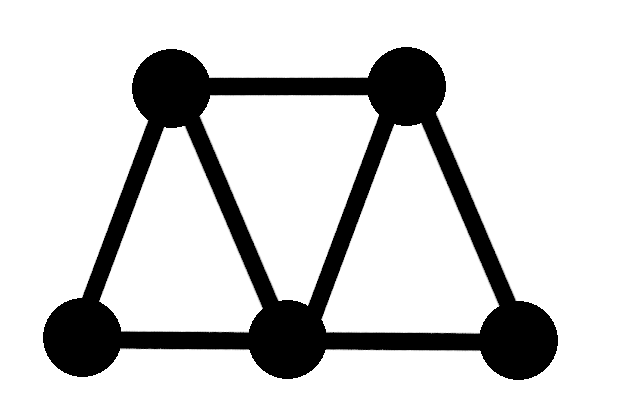
\includegraphics[scale = 0.4]{imagenes/base.png}
%		\end{center}
		\centering
		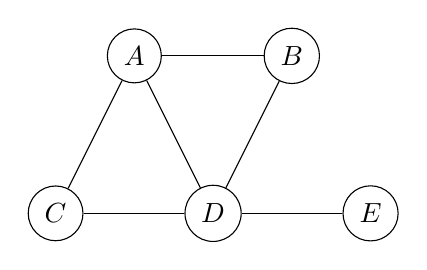
\begin{tikzpicture}
		\tikzstyle{normal}=[fill=white, draw=black, shape=circle];

		\node[normal] (C) at (0,0) {$C$};
		\node[normal] (D) at (2,0) {$D$};
		\node[normal] (E) at (4,0) {$E$};
		\node[normal] (A) at (1,2) {$A$};
		\node[normal] (B) at (3,2) {$B$};

		\draw (C) to (D) ;
		\draw (C) to (A) ;
		\draw (D) to (E) ;
		\draw (D) to (B) ;
		\draw (D) to (A) ;
		\draw (A) to (B) ;
        \end{tikzpicture}
	\end{minipage}
\end{frame}

\begin{frame}{Coloreo - \'Indice crom\'atico}
	\begin{minipage}{\anchoPagina \textwidth}
	\small
		Se define como \textit{\'indice crom\'atico} a la menor cantidad de colores distintos con los que se pueden colorear las aristas de un grafo $G$ de forma que todo par de aristas que inciden en un mismo v\'ertice tengan distinto color. Se lo nota $\chi'(G)$.
		\vspace{0.2cm}
        \begin{tcolorbox}[title=Propiedades]
        Sea $\mathcal{K}_n$ grafo completo de $n$ vértices:
        \begin{enumerate}
            \item $\chi'(\mathcal{K}_n) = n-1 = \Delta(\mathcal{K}_n)$ si $n$ es par.
            \item $\chi'(\mathcal{K}_n) = n = \Delta(\mathcal{K}_n)+1$ si $n$ es impar
        \end{enumerate}
        \end{tcolorbox}
        \vspace{0.2cm}
		\begin{tcolorbox}[title=Teorema de Vizing]
		Sea $G$ un grafo:
		
		$\Delta(G) \leq \chi'(G) \leq  \Delta(G) + 1$
		\end{tcolorbox}
	\end{minipage}
\end{frame}

\begin{frame}{Coloreo - Ejercicio 1}
	\begin{minipage}{\anchoPagina \textwidth}
		Se quieren usar torres existentes para transmisi\'on de ondas para celular. El problema es que dos torres que est\'an muy cerca (a una distancia menor que $d$ mts.) pueden interferirse si se utiliza la misma frecuencia para ambas. ¿Cu\'al es el menor n\'umero de frecuencias diferentes que hace falta usar en este caso para que no haya interferencia entre dos torres?
		
		Modelar el problema como un problema de coloreo.
	\end{minipage}
\end{frame}


\begin{frame}{Coloreo - Ejercicio 2}
	\begin{minipage}{\anchoPagina \textwidth}
		Supongamos que 11 equipos deben jugar entre s\'i todos contra todos una vez. Suponiendo que un equipo no puede jugar m\'as de un partido por d\'ia, ¿cu\'antos d\'ias son necesarios para jugar todos los partidos? Modelar este problema como un problema de coloreo de aristas y como un problema de coloreo de v\'ertices.
	\end{minipage}
\end{frame}

\end{document}

